%%%%%%%%%%%%%%%%%%%%%%%%%%%%%%%%%%%%%%%%  NuMI  %%%%%%%%%%%%%%%%%%%%%%%%%%%%%%%%%%%%%%%%%%%%%%%%%%%
\chapter{MINER$\nu$A Experiment}
\minitoc
\label{Cap:MnvExperiment}

\section{Introduction}
\label{Chap2:MnvExperiment:Intro}
MINER$\nu$A is a neutrino experiment that has as main goal measure the neutrino cross section on 6 different materials, such as lead (Pb), iron (Fe), water ($H_2O$), carbon (C), plastic scintillator and (CH) and Helium (He). This with the aim to use the obtained results to improve nuclear models which would be used in future neutrino oscillation experiments. The MINER$\nu$A detector was located in the MINOS Near Detector building (MINOS Hall) in the neutrino campus in Fermilab 100 m underground with the aim to remove the cosmic rays background in the line of the neutrino beam produced by NuMI. It was located upstream to the MINOS ND, MINER$\nu$A was not an magnetized detector, in this way MINER$\nu$A could use to MINOS ND as muon spectrometer, reducing the uncertainties of muon charge and momentum.  

The experiment starts to take data from 2009 to 2019. For the first 3 years (2009-2012) taking data with the mode Low Energy (LE) neutrino beam ($<E_\nu>=3$ GeV) and in the Medium Energy (LE) mode ($<E_\nu> = 6$ GeV) during the following years (2013-2019). The total number of Protons on Target (POT) that produced the neutrino beam were $16.1\times10^{20}$ in neutrino mode and $14.1\times10^{20}$ in the antineutrino mode. 

\section{NuMI Beam}
\label{Cap:MnvExperiment:NuMI}
The Neutrino at the Main Injector \cite{Numi} (NuMI) neutrino beam is a facility that has provided neutrinos to experiments such as MINOS\cite{MINOS}, COSMOS\cite{COSMOS}, MINER$\nu$A\cite{MINERvA}, ArgoNeut\cite{ArgoNeuT}, NOvA\cite{NOvA}, MINOS+\cite{MINOS+} and more recently ArgonCube 2x2\cite{twobytwo}.

The NuMI beam facility provides neutrino and antineutrinos to the different experiments colliding a proton beam of 120 GeV against a graphite target. The charged hadron produced are  focused by two to magnetic horns. Depending the direction of the electrical current in the horns neutrinos or antineutrinos are produced in the resulted beam. The horn focused the hadrons throughout the decay pipe and during the travel most part of these hadrons decays in a neutrino and other charged particles. Most part of the remnant charged particles are absorbed by the rock, obtaining in this way an intense neutrino beam passing through the rocks.  

\begin{figure}[!htb]
\centering
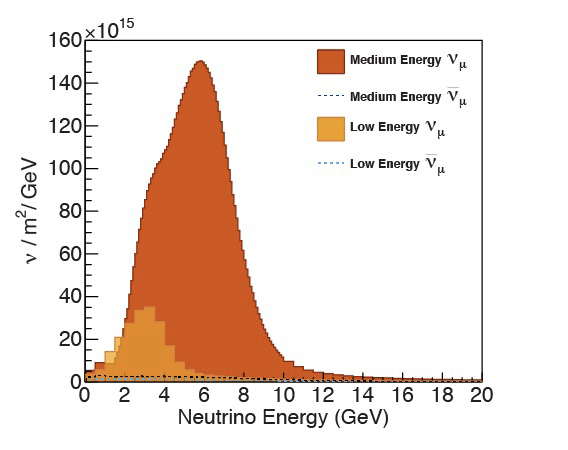
\includegraphics[scale=0.38]{Figures/Chapter2/fluxantineutrino.png}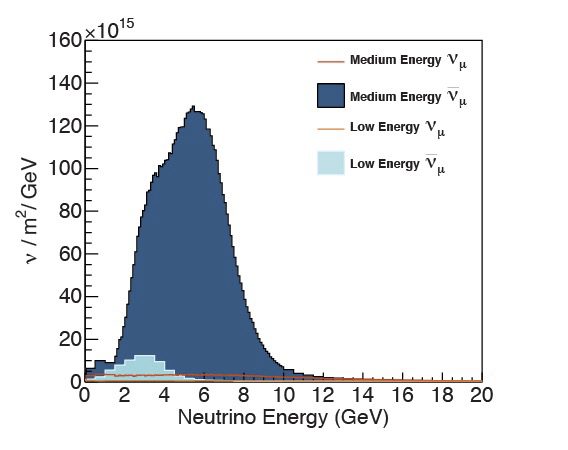
\includegraphics[scale=0.38]{Figures/Chapter2/fluxneutrino.png}
        \caption{Absolute flux for the neutrino mode (left) and the antineutrino mode (right) for the LE and ME eras.} 
\label{fig:MnvExp:NuMI:Flux}
\end{figure}

During the period of 2009 to 2012 the MINER$\nu$A detector collected data in the the Low Energy (LE) mode of the NuMI beam, with a $<E_\nu> = 3$ GeV. For the period of 2013 until 2019 it collected data in the Medium Energy (ME) mode, with a $<E_\nu> = 6$ GeV.  In the \textbf{Figure} \ref{fig:MnvExp:NuMI:Flux}.



\subsection{NuMI Design}

The NuMI beam uses the proton beam produced by the Fermilab Main Injector with an energy of 120 GeV. The proton beam starts accelerating hydrogen ($H^-$) ions using a radio-frequency quadrupole until 750 KeV. In the second stage, the ions are accelerated by a linac from 750 KeV to 400 MeV. The ions are passed through a thin carbon foil to removes the electrons from the $H^-$ obtaining just protons. 

\begin{figure}[!h]
\centering
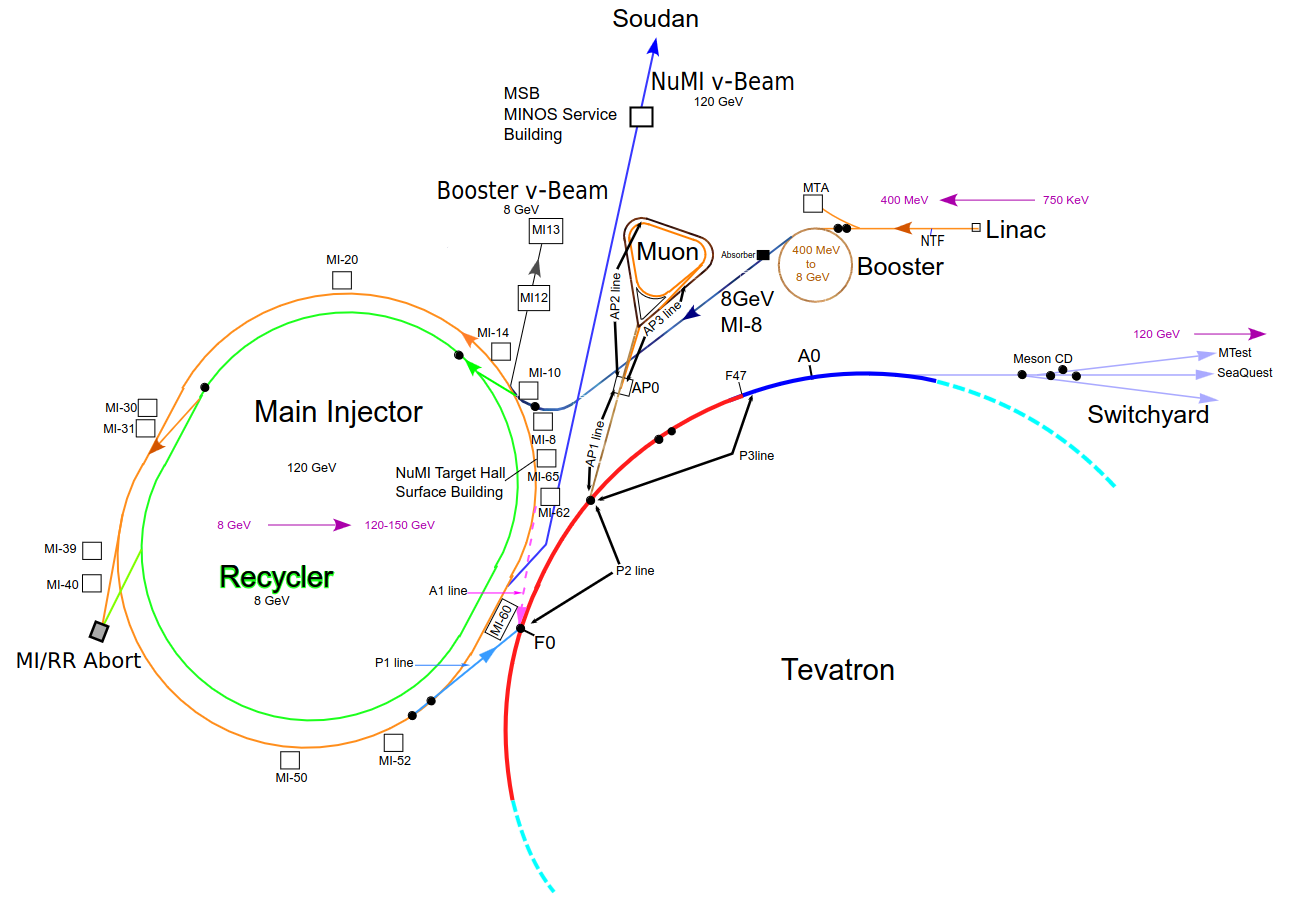
\includegraphics[scale=0.29]{Figures/Chapter2/AcceleratorComplex.png}
        \caption{Schematic of the Fermilab Accelerator complex. Image from \cite{Numi}.} 
\label{fig:MnvExp:NuMI:SchematicMainInjector}
\end{figure}

In the third stage the protons pass to the Booster, it is a 75 m radius synchrotron accelerator that accelerates the protons from 400 MeV to 8 MeV, at the same time it groups the protons in 1.6 $\mu s$ of long batches. 

The last stage of acceleration is on the Main Injector, it is a proton synchrotron 7 times the circumference of the booster. It accelerates the protons from 8 GeV to 120 GeV of energy. The beam produces is has Gaussian shape with a $\sigma =$ 1.1 mm, with a \textit{Cycle Time} = 1.87 s and 10 $\mu s$ beam spill duration. In the  \textbf{Figure} \ref{fig:MnvExp:NuMI:SchematicMainInjector} all the stages of acceleration are shown.

A portion of the proton spills are used by NuMI to produce the neutrino beam, the beam is bent in direction to the NuMI Target Hall. Here the protons are steered to a graphite target. The interaction of the protons with the graphite target produce an hadronical shower where the charged hadrons are focused by two parabolic magnetic horns in direction to the decay pipe. Depending of the current orientation of the current in the pipe, the neutrino mode or antineutrino mode beam can be chosen. The major portion of the hadrons produced are pions and kaons, the predominant decay channel for the pions is $\pi^+ \longrightarrow \mu^+ + \nu_\mu$ and $K^+ \longrightarrow \mu^+ + \nu_\mu$ giving a $\nu_\mu$ beam, for the case of the antineutrino beam, the negative hadrons are focused obtaining as result $\Bar{\nu}_\mu$. 


\begin{figure}[!htb]
\centering
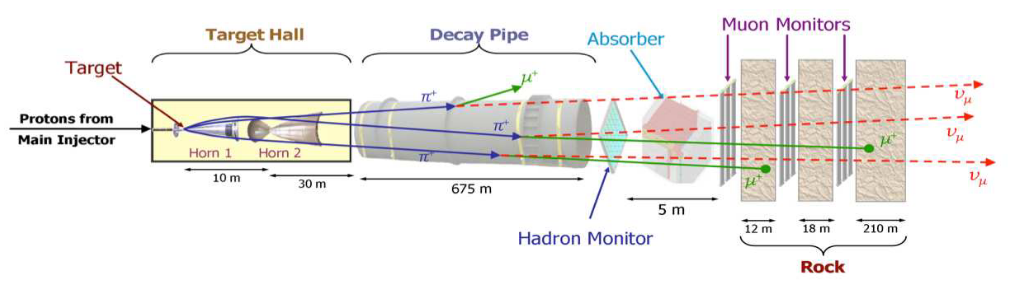
\includegraphics[scale=0.38]{Figures/Chapter2/NuMIScketch.png}
        \caption{Schematic of the Fermilab NuMI Beam. Image from \cite{Numi}.} 
\label{fig:MnvExp:NuMI:SchematicNuMIBeam}
\end{figure}

When the horns focus positive hadrons, the beam consist of 93\% of $\nu_\mu$, 6\% $\Bar{\nu}_\mu$ and 1\% $\nu_e + \Bar{\nu}_e$. In the \textbf{Figure} \ref{fig:MnvExp:NuMI:NuMIBeamComponents} We can observe the different components of the neutrino beam for the neutrino mode in the ME era. 
\begin{figure}[!htb]
\centering
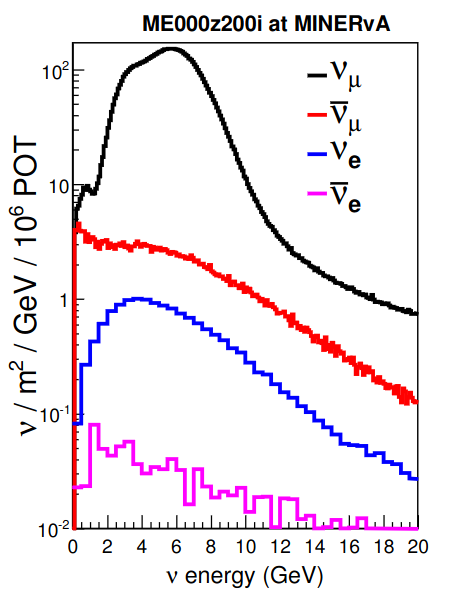
\includegraphics[scale=0.4]{Figures/Chapter2/NuMIbeamComponents.png}
        \caption{Neutrino beam components. Image from \cite{LeoThesis}.} 
\label{fig:MnvExp:NuMI:NuMIBeamComponents}
\end{figure}


\subsubsection{NuMI components}
In this subsection, the components of the NuMI beam are described in more detail the components of NuMI.

\textit{NuMI Target Hall}

It is a complex that contains the major part of the components to produce the neutrino beam. In addition to containing a large part of the NuMI instrumentation, it has the roll to shield the high levels of radioactivity, heating and thermal shock that is produced while the beam is on.  

The Target Hall is located in Fermilab approximately 41 m underground, 69 m of length, 8.1 m wide and 12.5 m high. Initially, the beam was designed with the goal to sent neutrinos to MINOS Near (in Fermilab) and Far (in Soudan Laboratory, Minnesota) detectors, therefore, the neutrino beam is bend $3.343^o$ downwards.  

\begin{figure}[!htb]
\centering
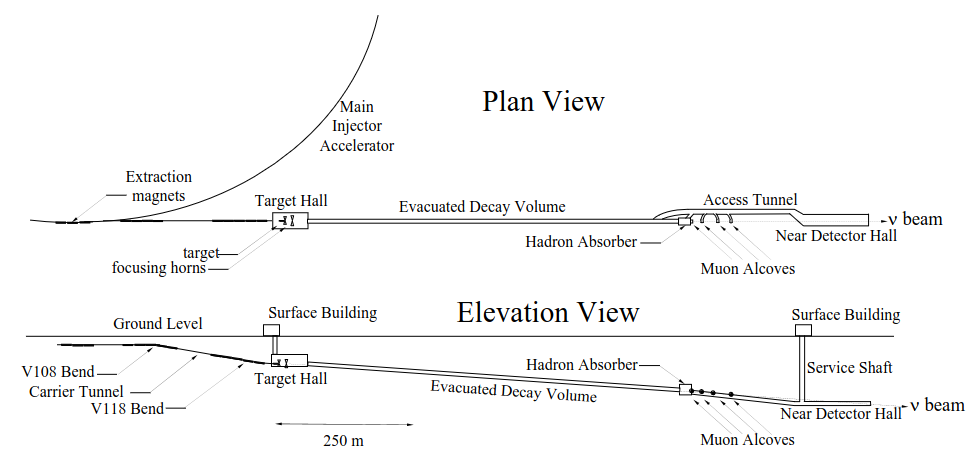
\includegraphics[scale=0.4]{Figures/Chapter2/NuMIFacilityViews.png}
        \caption{Views of the NuMI beam complex. Image from \cite{Numi}.} 
\label{fig:MnvExp:NuMI:NuMIviews}
\end{figure}

The instrumentation in the Target Hall allows to fix the different beam energy configurations. The energy configuration depends of the distance of between the horns and the target, therefore, it is necessary a central chase. In this chase the components and instrumentation of the beam can be moved depending the beam configuration, at  the same time the chase is also part of the cooling system. 

The cooling system recirculate air in the different components with a capacity of 240 kW of cooling. This system removes the heat for a correct functioning of the beam. For the horns, the cooling system use water to control the temperature.

The NuMI Target Hall has a crane that allow to move, repair and replace equipment remotely. This also has a Work Cell that is a shielded facility where the personnel can access and work in the maintenance of the equipment. 

\textit{The NuMI Target}

The NuMI target is designed to support until 400 kW power without disintegrated, at the same time it should produce the maximizing the production of hadrons and reducing the interactions of the hadrons with the target. So the target can not be very robust because it increase the interaction of the hadrons with the target. The design of the target have to consider that it have to have a high thermal conductivity, it should be available to maintain its mechanical condition at the high temperature conditions, withstand long operational journeys and radiation damage. 

The NuMI Target is made of graphite of type ZXF-5Q with a density of 1.78 g/cm$^3$ \cite{Numi}. It consists of 48 segments of 24 mm long (in beam direction)$\times$ 63 mm tall $\times$ 7.4 mm wide The total length of the target is 95.38 cm, spaced 0.3 mm \cite{BenThesis}.

\begin{figure}[!htb]
\centering
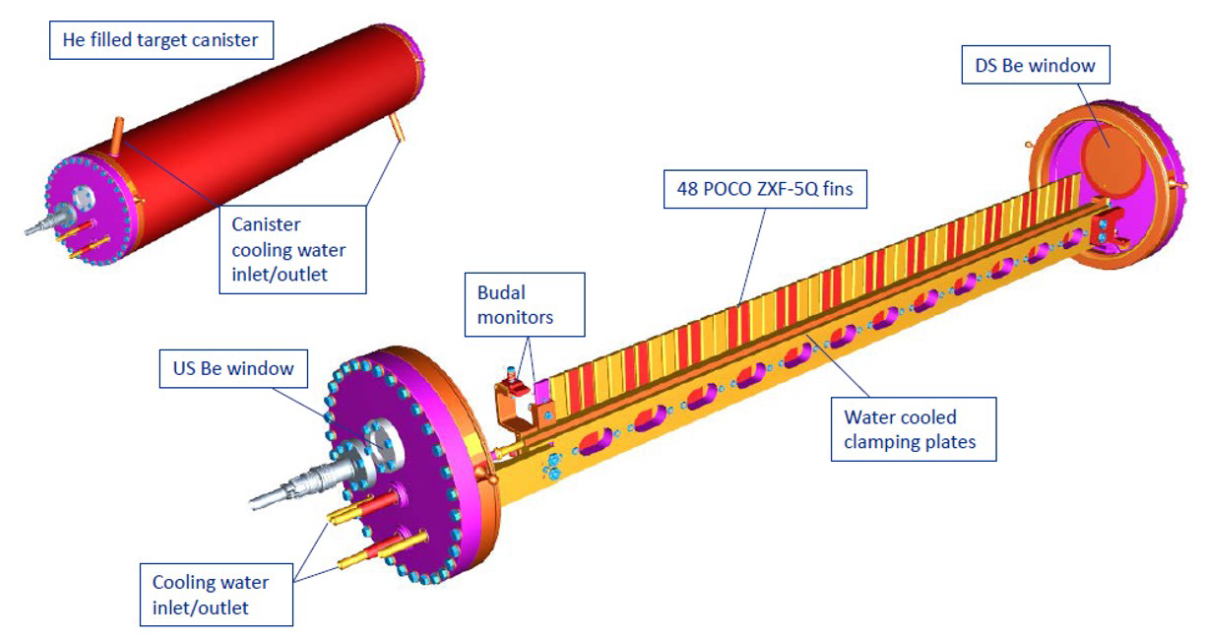
\includegraphics[scale=0.33]{Figures/Chapter2/NuMITarget.png}
        \caption{NuMI Target design for the ME era. Image from \cite{NuMITarget}.} 
\label{fig:MnvExp:NuMI:NuMITarget}
\end{figure}

The NuMI Target is isolated by vacuum and surrounded by two stainless steel tubes that carry the water coolant. These are counted in an aluminum canister filled with He. The entrance and the exit if the beam in the target vessel are made of beryllium. The Budal monitors \cite{Budal} are used to check the alignment of the target respect to the beam. 

\textit{The Target/Baffle Carrier}

The Baffle \cite{NOvATDR} protects the neck of the horn and the cooling hardware form the miss-steered beam pulses. It consist in a 1.5 long graphite core with 57 mm of diameter encased in an aluminum tube. It has an 13 mm diameter center hole along the the rod, where the proton beam passes. 

The Target and the Baffle are mounted in a structure called \textit{Target/Baffle Carrier}. This brings mechanical support, connections to the cooling system and connection to the electrical lines. This structure has installed positioning motors that allow motion of the target vertically and horizontally. 

 \begin{figure}[!htb]
\centering
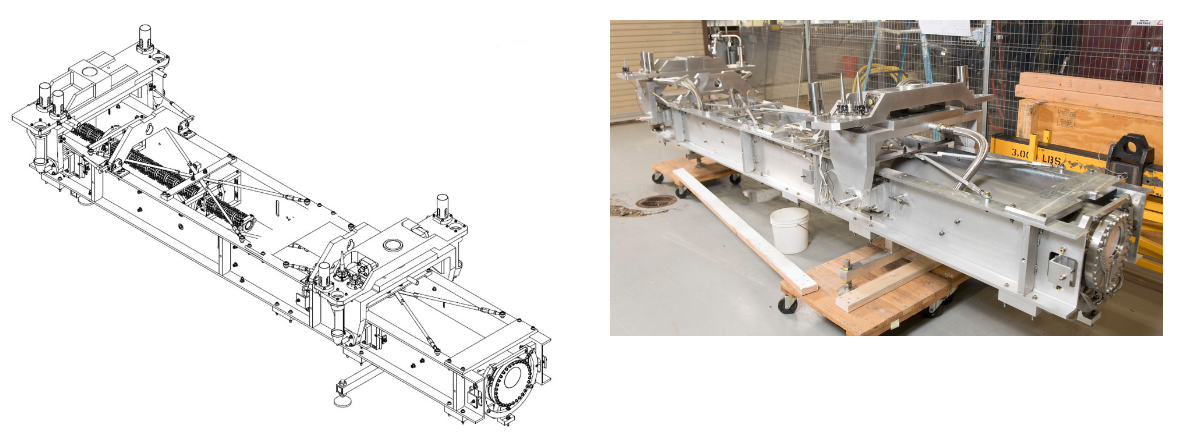
\includegraphics[scale=0.33]{Figures/Chapter2/TargetCarrier.png}
        \caption{Left, NuMI Target/Baffle design. Right, picture of the NuMI Target/Baffle carrier with the target installed. Image from \cite{NuMITarget}.} 
\label{fig:MnvExp:NuMI:NuMITargetCarrier}
\end{figure}

\textit{Magnetic Horns}

The magnetic horns have as their main objective maximize the neutrino flux focusing the secondary particles produced in the target on direction of the detectors, at he same time that can be used to select the neutrino energy spectrum. In the \textbf{Figure} \ref{fig:MnvExp:NuMI:HornsFocusSystem} shows a diagram of how the trajectory of the particles are modified by the horns. 

\begin{figure}[!htb]
\centering
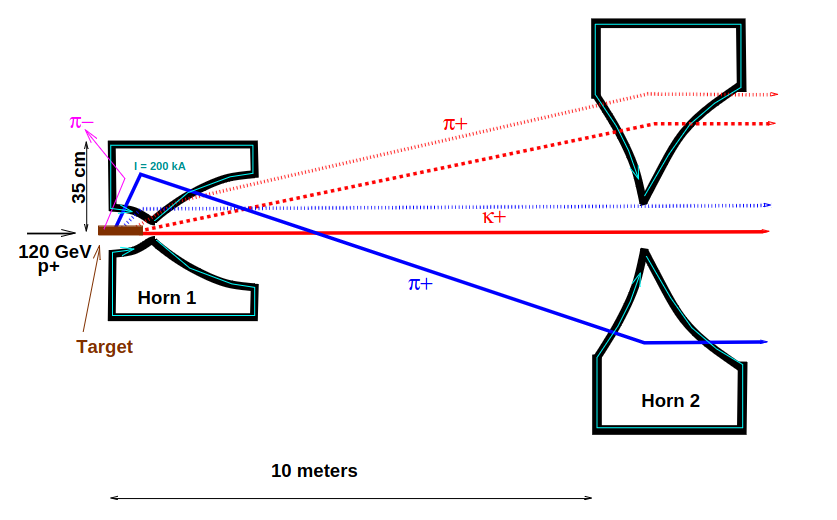
\includegraphics[scale=0.33]{Figures/Chapter2/HornsFocusSystem.png}
        \caption{Schematics of the Horn 1 of Horn 2 modifying the trajectory of the particles. Depending the current direction of the current in the horns the $\nu_\mu$ or $\Bar{\nu}_\mu$ mode can be selected. Image from \cite{Numi}.} 
\label{fig:MnvExp:NuMI:HornsFocusSystem}
\end{figure}

The horns are made of an alloy of nickel-plated aluminum in the inner conductor and for the outer conductor it use anodized aluminum. The inner conductor of the Horn 1 is 2 mm of thickness and 3 mm for the Horn 2 in the most part of the regions. The thickness of the horns should be such that it allows the passage of a large electric current and avoiding the absorption or interaction of the secondary hadrons with the horns. The double paraboloidal shape of the horns produce a toroidal magnetic field where the intensity of the magnetic field falls as the inverse of the radium between the inner and the outer conductors. The expected magnetic field in the longitudinal axis of the horns should be zero and in the maximum transverse field is 3T. To produce the magnetic field in the horns, a pulsed 200 kA of current pass through them with a duration of 2.3 ms.

The high current and the interaction of the hadrons with the horns increases the heat of those, hence, it is necessary to have a cooling system to guaranty a good operation during long periods of time. The cooling system spray water to the inner conductor keeping the temperature below 100 C. 

\begin{figure}[!htb]
\centering
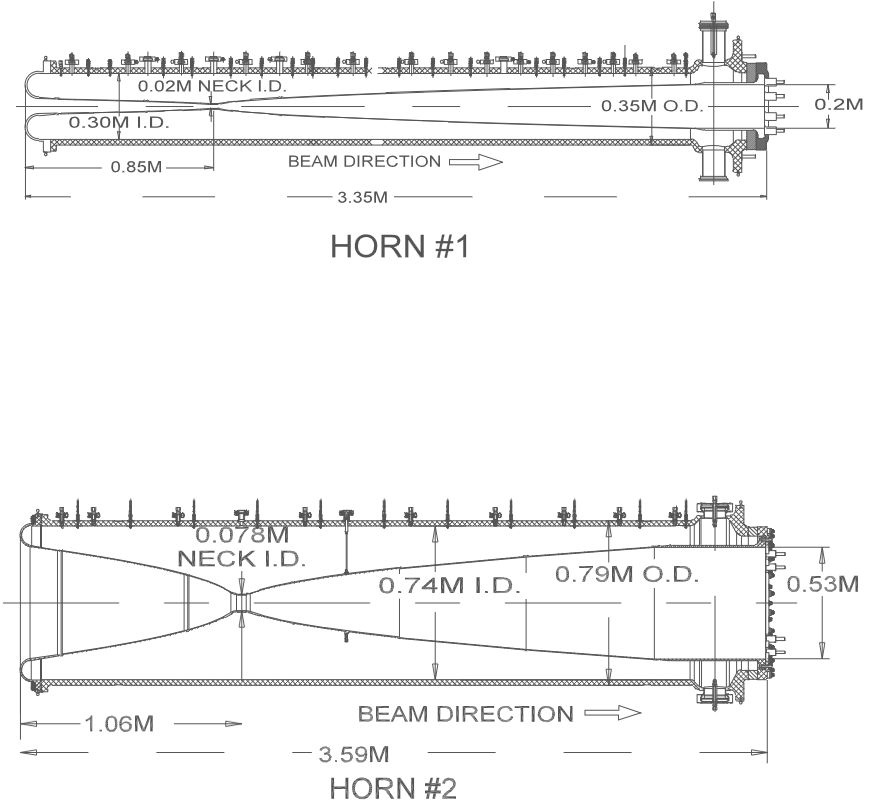
\includegraphics[scale=0.33]{Figures/Chapter2/SchematicMagneticHorns.png}
        \caption{Schematics of the Horn 1 of Horn 2. In the images the dimensions and longitudinal cut of the horns are shown. Image from \cite{Numi}.} 
\label{fig:MnvExp:NuMI:NuMIHornsSchematic}
\end{figure}

Depending of the momentum and the charge of the hadrons, the effects of the horns on the hadrons can be categorized as follow:

\begin{itemize}
    \item \textit{Deflected}: Selecting the direction of the current, the horns can be used to focus only positive or negative hadrons. This allows to select between $\nu$ or $\Bar{\nu}$ beam. It means that when the $\nu$ mode is selected, the negative particles are deflected by the horns, and vise-versa.
    \item \textit{Unfocused} : These are the hadrons that pass very close to the necks of the horns and the trajectory of this particles is not modified by the horns. The most part of these are hadrons with a momentum above to 15 GeV. 
    \item \textit{Underfocused} : These are hadrons that have to pass by the two horns to be focused. The range of the momentum for the hadrons is between 5 GeV and 15 GeV.
    \item \textit{Overfocused}: These are particles that pass throughout the horn 1 and horn 2. Unlike of the underfocused, these are hadrons with a momentum below to the 5 GeV. 
    \item \textit{Horn-1-only}: These are particles that are corrected only by the Horn 1 and that pass throughout the neck of the Horn 2. The transversal momentum of these hadrons usually is above to the 0.2 GeV.
    \item \textit{Horn-2-only} : These are hadrons that pass throughout the neck of the Horn 1 and that are only corrected by the Horn 2. The momentum of these hadrons is between the range of 9 GeV and 15 GeV.
\end{itemize}

\begin{figure}[!htb]
\centering
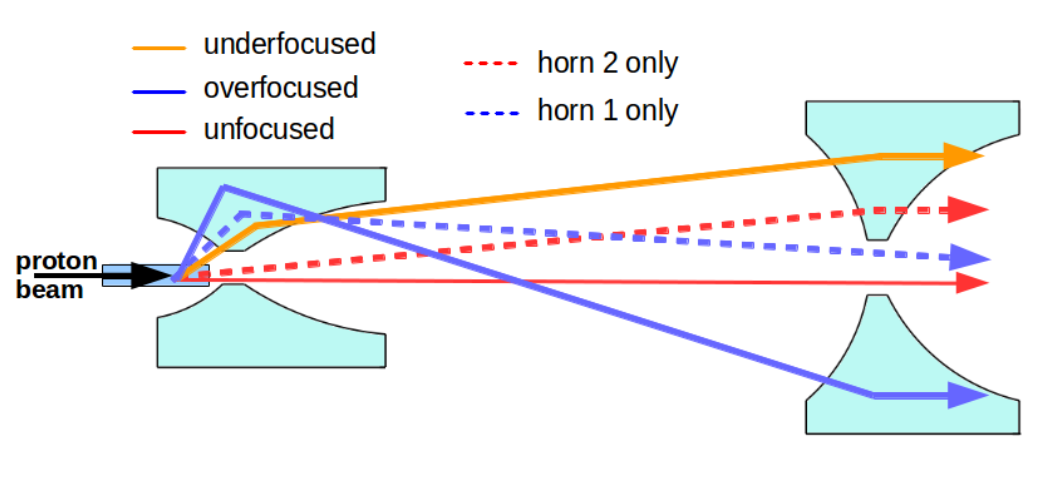
\includegraphics[scale=0.33]{Figures/Chapter2/FocusingComponents.png}
        \caption{Image where the categories of focusing effects are represented. Image from \cite{LeoThesis}.} 
\label{fig:MnvExp:NuMI:NuMIFocusingComponents}
\end{figure}

The focused hadrons with the largest momentum are the hadrons that have a small component of the transversal momentum respect to the proton beam. Therefore, if the horns are close the number of focused hadrons with low momentum increase respect to the high momentum, and vise-versa. Considering this fact, the distance between the horns can be used to select the spectrum energy of the focused hadrons, resulting in a selection of the spectrum of the neutrino beam. The NuMI beam can be used in three energy configurations. Low Energy (LE) where the $<E_\nu>=3.5$ $GeV$, Medium energy (ME) where $<E_\nu>=7$ $GeV$ and High Energy where the $<E_\nu> = 14$ $GeV$\cite{BeamOptics}. 

\begin{figure}[!htb]
\centering
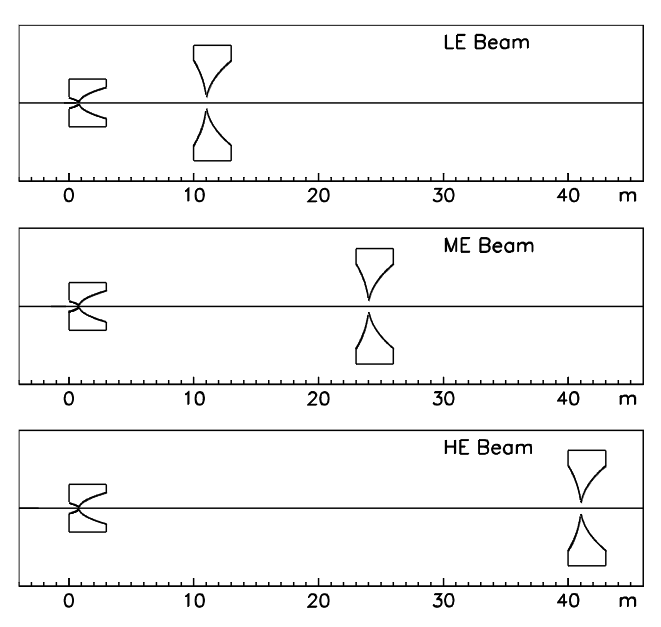
\includegraphics[scale=0.4]{Figures/Chapter2/HornsDistance.png}
        \caption{In this image the distance between the horns for the different energy configurations is shown. Image from \cite{BeamOptics}.} 
\label{fig:MnvExp:NuMI:NuMIHornDistance}
\end{figure}

\begin{figure}[!htb]
\centering
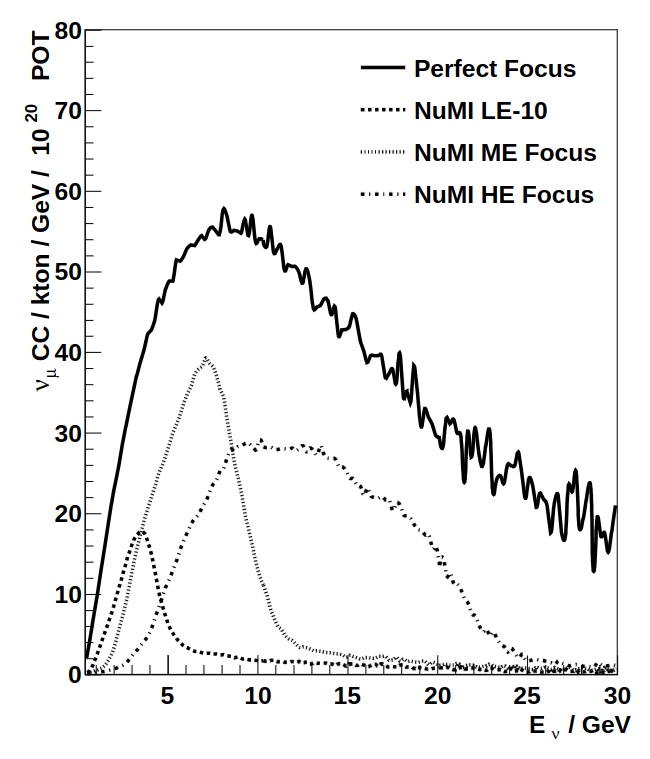
\includegraphics[scale=0.3]{Figures/Chapter2/nuAllSpectrums.png}
        \caption{In this graph, the simulated neutrino spectrum for the different neutrino neutrino energy beam configurations. Image from \cite{Numi}.} 
\label{fig:MnvExp:NuMI:Neutrino spectrum}
\end{figure}

\textit{Decay Pipe}

After to focus the secondary hadrons, these pass throughout the \textit{Decay Pipe}. Here, the most part of the hadrons decay and produce the neutrino beam. The goal of the Decay Pipe is to reduce the interactions of the hadrons with the surroundings. To reduce the interactions inside of the Decay Pipe is produced conditions of low density environment. 

The dimensions of the Decay Pipe are 2 m of radius $\times$ 645 m in length. It is surrounded by concrete to reduce the radiation effects in the groundwater. The Decay Pipe is designed to work at internal vacuum conditions and with other low density gases such as helium. 

The collisions of particles with the pipe heat the structure, with the aim to reduce the temperature and to guarantee a long operations of the facility, a cooling system is installed in the pipe. This allow to keep a temperature bellow to the 50 C. 

\textit{Absorber}

Downstream to the Decay Pipe, a structure of aluminum, steel and concrete is installed to stops the protons that did not interact with the NuMI Target and other remnant beam particles, this structure is the absorber. The absorber is an essential component to reduce the levels of radiation and to avoid the groundwater from radiation. The deposition of the energy of the particles generate a temperature increment of the absorber, hence this has a cooling system to maintain the temperature bellow to 50 C. 

\textit{Muon Shield} 

The Muons shield is the last part of the NuMI beam, this works as a shield for the detectors situated in the MINOS Hall from the muons produced in the decay of the mesons in the production of the neutrino beam. This consist in 240 m of dolomite rock that stops the muons. 

\pagebreak



\section{MINER$\nu$A Detector}
\label{Cap:MnvExp:MnvDetector}

The Minerva detector is a fine-grained detector that use as active detection material plastic scintillator to detect the charged particles produced in the neutrino interactions. The design of the detector allows to make a 3D spatial reconstruction at the same time that allows to make a reconstruction of the deposited energy by calorimetric and range techniques. 

The MINER$\nu$A experiment physics goals include produce the measurement of the inclusive and exclusive cross section studies of diverse types of interactions, therefore a good energy reconstruction for low and high energy Final States Interaction (FSI), particle identification and the understanding of multiple interactions in a single beam spill are necessary. Considering the previous points, the detector was design to use different passive nuclear targets, having as active detection material plastics scintillator, that it is a low density active detection material that allows to make a good reconstruction of low energy events. A large portion of the detector is filled of this material with the aim to reconstruct the multi-particle final state at the same time that is surrounded by a electromagnetic (ECAL) and hadronic (HCAL) calorimeters to contain all the particles generated in the interaction. The muons are particles the are not easy to stop, for this reason the detector was situated upstream of the MINOS Near detector with the aim to use it to reconstruct the momentum and determine the charge of the muons produced in the neutrino interactions inside of MINER$\nu$A.


\begin{figure}[!htb]
\centering
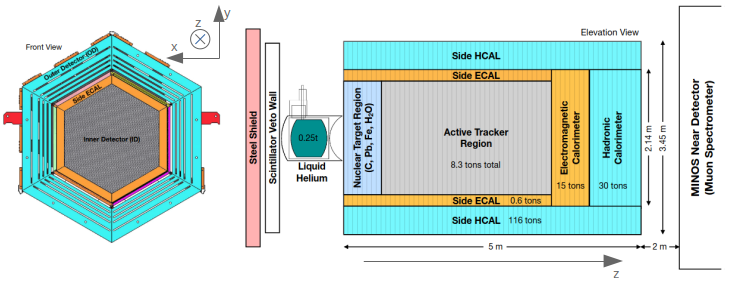
\includegraphics[scale=0.5]{Figures/Chapter2/DetectorScheme.png}

        \caption{Scheme of the MINER$\nu$A detector. . Figure from \cite{ALIAGA2014130}} 
\label{fig:MnvExp:MnvDetector:Scheme}
\end{figure}

The MINER$\nu$A coordinate system is set as follow. The origin of the plane X-Y is situated in the center of the MINER$\nu$A hexagon. The Z axis origin is situated 1200 cm downstream of the MINOS detector, this goes along the center of the MINER$\nu$A detector. The direction of the neutrino beam point 3.34$^o$ downward in the Y-Z plane. 

In the transversal direction of the detector it is segmented in the Inner Detector (ID), where are contained the active tracking planes, nuclear targets, downstream Electromagnetic Calorimeter (ECAL) and the Hadronic Calorimeter (HCAL); and the Outer Detector (OD) that consist of a steel frame with plastic scintillator embedded that works as HCAL and mechanical support to the planes.   

\subsection{Active Tracking planes}
\label{Cap:MnvExp:MnvDetector:ActiveTrackingPlanes}

The detector has active and passive nuclear targets. The active nuclear targets are triangular plastic scintillator strips. When a charge particle pass throughout a scintillator materials, the particle transfers part of its energy to the material, after short time it becomes de-energized emitting light a pulse\cite{DetectionTechniques}. 

The triangular scintillator stripes have a base of 3.3 cm and 1.7 cm height, the length of the strips varies between 85 cm and 170 cm. These are composed of polystyrene doped with  2,5-diphenyloxazol (PPO) and 1,4-bis(5-phenyloxazol-2-yl) benzene (POPOP). These two materials works as weave length shifters. The polystyrene emits light in the far UV region, the PPO absorbs the light en re-emits it in the region of the near UV and then the POPOP absorbs this light and emits it as visible blue light. Along of center of the scintillator strips there is placed an optical fiber that absorbs the blue light and then this re-emits the light on green in the ends of the fiber. The reason for that the light have to be shifted is because the the photo-detectors that transform the light to electrical signals works more efficiently with green light, this process is explained with more detail on the \textbf{subsection} \ref{Cap:MnvExp:MnvDetector:PhotoDetectionSystem}. The scintillator strips are painted with white EJ-510 $TiO_2$ Eljen paint\cite{StripsPaint}. 


\begin{figure}[!htb]
\centering
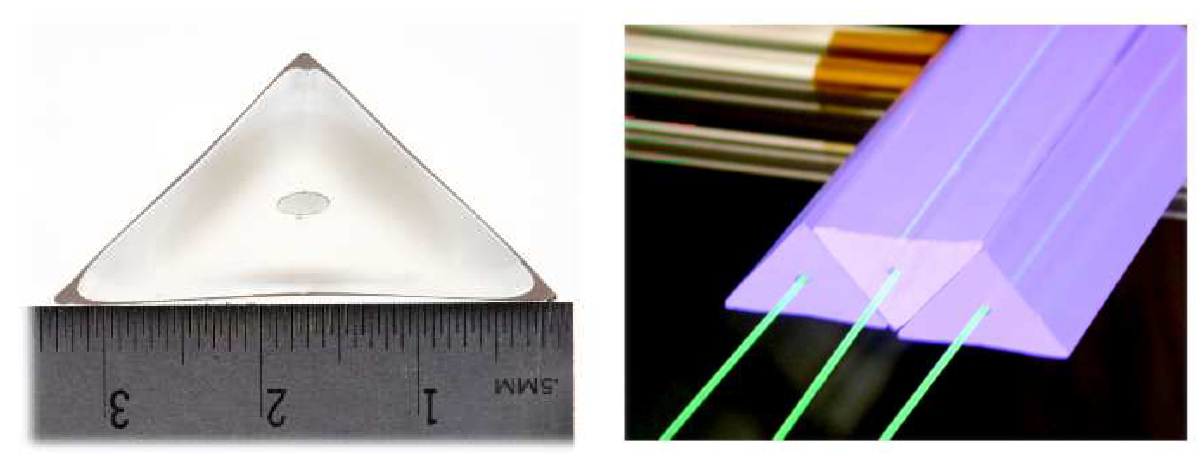
\includegraphics[scale=0.3]{Figures/Chapter2/ScintStripes.png}

        \caption{Images where the plastics scintillators are shown. Figure from \cite{MINERvA}} 
\label{fig:MnvExp:MnvDetector:TriangularStripes}
\end{figure}

The scintillator strips are arranged as is observed in the \textbf{Figure} \ref{fig:MnvExp:MnvDetector:StripsArrange}. The tracking planes are composed of two plastic scintillator planes. On each plane there are 127 strips glued using 3M-DP190 translucent epoxy. The planes are also insulated optically from the exterior. 

\begin{figure}[!htb]
\centering
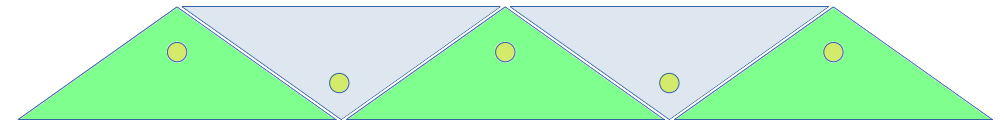
\includegraphics[scale=0.3]{Figures/Chapter2/stripsArrange.png}

        \caption{Scheme that shows how are arranged the scintillator strips to compose the tracking planes.} 
\label{fig:MnvExp:MnvDetector:StripsArrange}
\end{figure}

The tracking planes can be oriented 1 of X, U or V configuration. The orientation of the strips in the X configuration is $90^o$ respect to the horizontal. For the U and V are rotated $60^o$ and $-60^o$ respectively, taking as reference the X orientation, in the \textbf{Figure} \ref{fig:MnvExp:MnvDetector:PlanesOrientations} three schemes of the orientation configurations are shown. The three orientations are used to avoid reconstruction ambiguities for events that contain two particles and deposit energy in orthogonal planes. For the shape and the arrangement of the scintillator strips in the tracking planes, each time that a charge particle pass throughout a plane most part of the particles will interacts with two scintillator strips. 

\begin{figure}[!htb]
\centering
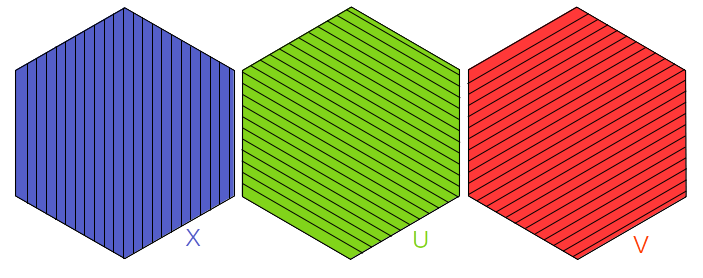
\includegraphics[scale=0.4]{Figures/Chapter2/PlanesOrientation.png}

        \caption{Scheme with that shows the different tracking modules orientations.} 
\label{fig:MnvExp:MnvDetector:PlanesOrientations}
\end{figure}

The planes are grouped in tracking modules, these consist of two tracking planes XU or XV. The modules are stacked in the pattern XUXV, this arrange allows a 3D reconstruction of the charged particles produced by the neutrino interactions that pass through the detector. In the \textbf{Figure} \ref{fig:MnvExp:MnvDetector:TrackingModules} shows a representation of charged particle passing throughout the tracking modules. 

\begin{figure}[!htb]
\centering
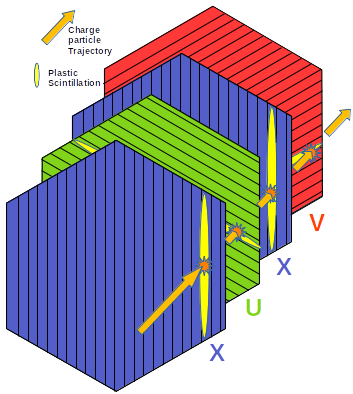
\includegraphics[scale=0.5]{Figures/Chapter2/TrackingModules.png}

        \caption{Scheme where the arrangement of the tracking modules is shown. In the figure is represented how a charged particle produce a signals in the planes.} 
\label{fig:MnvExp:MnvDetector:TrackingModules}
\end{figure}

All the planes are rounded by and hexagonal lead frames that plays the role of ECAL. They are framed by a steel hexagonal frame that bring mechanical support to the hole plane and it is an HCAL. The ECAL and the HCAL that rounds the tracking planes are shown in the \textbf{Figure} \ref{fig:MnvExp:MnvDetector:Scheme}.

\subsection{MINERvA detector Regions}
\label{Cap:MnvExp:MnvDetector:MnvDetectorRegions} 

\begin{itemize}
    \item \textit{Veto wall}

    The Veto Wall is located upstream of the MINER$\nu$A detector, this consist in a steel plate of 5 cm of thickness followed by a plate of plastic scintillator. This section of the detector is used to detect the muons that are produced by the interaction of the neutrino beam with the dolomite rock of the muon absorber. These muons are commonly called \textit{rock muons}.

    \item \textit{Nuclear Targets Region}

    Nuclear Target Region is composed of active and passive targets. The passive materials are Liquid Helium ($He$), Carbon ($C$), Lead ($Pb$), Water ($H_2O$) and Steel ($Fe$). In the \textbf{Figure} \ref{fig:MnvExp:MnvDetector:TargetRegion} the order of how where collocated the planes for passive and active materials in the target region is shown. The C, Pb, $H_2O$ and Fe targets ,in the same way that the active tracking planes, are supported by the ECAL and HCAL.
    
    \begin{figure}[!htb]
    \centering
    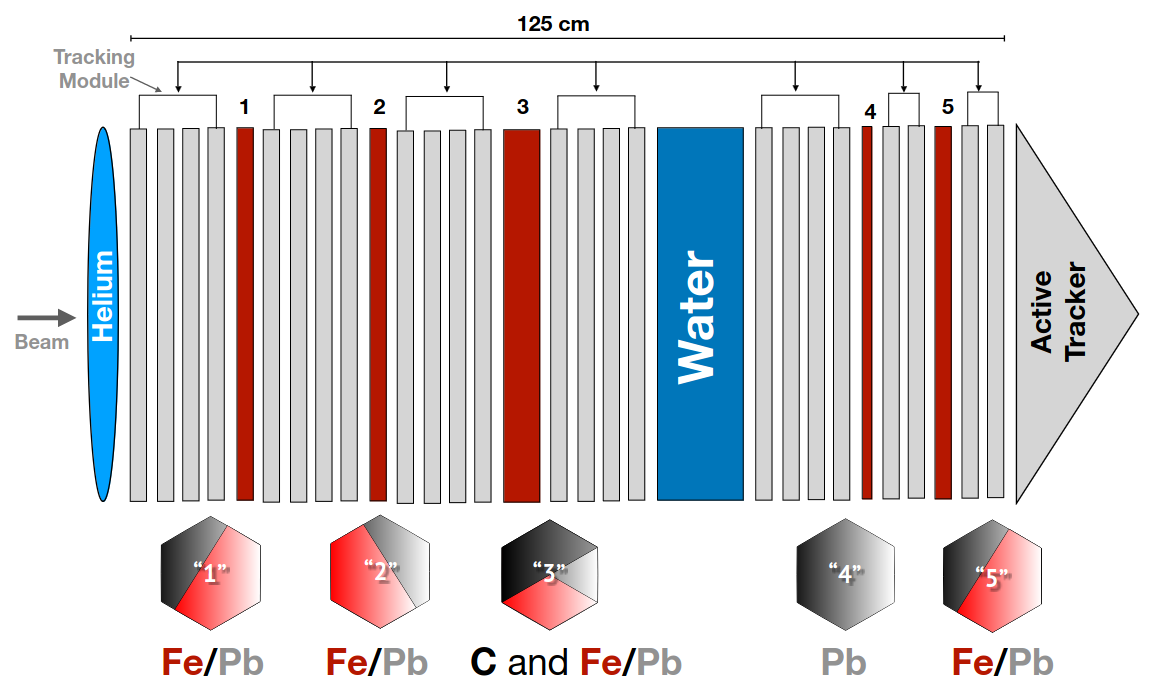
\includegraphics[scale=0.35]{Figures/Chapter2/TargetRegion1.png}

        \caption{Scheme that shows the order that are arranged the target planes in the Target Region. The target region is composed for a cryostat with the Liquid He target, 5 solid targets and the water target. Figure from \cite{MarvinThesis}} 
    \label{fig:MnvExp:MnvDetector:TargetRegion}
    \end{figure}
    
    The He target cryostat is located downstream from the veto wall. This target is capable to contain 2300 L of Liquid He, it was filled during the last parts of the run \cite{ALIAGA2014130}. The other targets are located upstream from the He target. With the aim to localize the neutrino interaction vertex, the nuclear targets planes are located between to tracking modules as shown in the \textbf{Figure} \ref{fig:MnvExp:MnvDetector:TargetRegion}, except for the thin lead target, that only 1 tracking module is located upstream. After the fifth target, the modules of the tracker region starts. In the \textbf{Tables} the information about the composition of the targets is descrived. 

    \begin{table}[!htb]
        \centering
        \begin{tabular}{c c c c c c c c}
            \textbf{Material} & \textbf{Density} & \textbf{C(\%)} & \textbf{Si (\%)} & \textbf{Mn (\%)} & \textbf{Fe (\%)} & \textbf{Cu (\%)} & \textbf{Pb (\%)} \\ 
             & \textbf{(g/cm$^2$)} & & & & & & \\ \hline
            Steel & 7.83±0.03 & 0.13 & 0.2 & 1.0 & 98.7 & - & - \\
            Lead & 11.29±0.03 & - & - & - & - & 0.05 & 99.95\\
            Graphite & 1.74±0.01 & >99.5 & - & - & - & - & - \\ \hline
        \end{tabular}
        \caption{In this table the density and element composition for the solid nuclear targets is shown. Table from \cite{ALIAGA2014130}}.
        \label{tab:Chapter2:Detector:NuclearTargetsComposition}
    \end{table}

    \begin{table}[!htb]
        \centering
        \begin{tabular}{c c c c c c}
            \textbf{Target} & \textbf{z-location} & \textbf{Thickness} & \textbf{Fiducial area} & \textbf{Fiducial mass} & \textbf{Total mass}  \\ 
             & \textbf{(cm)} & \textbf{(cm)} & \textbf{cm$^2$} & \textbf{(kg)} & \textbf{(kg)} \\ \hline
            1-Fe & 452.5 & 2.567±0.006 & 15999 & 322 & 492 \\ 
            1-Pb & 452.5 & 2.578±0.012 & 9029 & 263 & 437 \\
            2-Fe & 470.2 & 2.563±0.006 & 15999 & 321 & 492 \\ 
            2-Pb & 470.2 & 	2.581±0.016 & 9029 & 263 & 437 \\
            3-Fe & 492.3 & 	2.573±0.004 & 7858 & 158 & 238 \\ 
            3-Pb & 492.3 & 2.563±0.004 & 3694 & 107 & 170 \\
            3-C & 492.3 & 7.620±0.005 & 12027 & 160 & 258 \\ 
            Water & 528.4 & 17–24 & 25028 & 452 & 627 \\
            4-Pb & 564.5 & 0.795±0.005 & 25028 & 225 & 340 \\
            5-Fe & 577.8 & 1.289±0.006 & 15999 & 162 & 227 \\ 
            5-Pb & 577.8 & 1.317±0.007 & 9029 & 134 & 204 \\ \hline
        \end{tabular}
        \caption{The z position, thickness, fiducial area, fiducial mass and total mass of the nuclear targets are shown. The z-location is determined according the coordinate system described in the text. Table from \cite{ALIAGA2014130}. }
        \label{tab:Chapter2:Detector:Sizes}
    \end{table}

    The water target, unlike the solid targets, is hold by a circular frame. The diameter of this frame is larger that the MINER$\nu$A inner detector size. The water container is made of two Kevlar\textsuperscript \textregistered sheets. The internal hydrostatic pressure of water deform the shape of the water container, for that reason the water target is not well defined. The geometry of the targets is part of the parameters of the particle simulation it is necessary to have a good  approximation of the shape of the targets, with the aim to obtain the best approximation to the water target shape, the container shape was simulated via finite element analysis. 

    \begin{figure}[!htb]
        \centering
        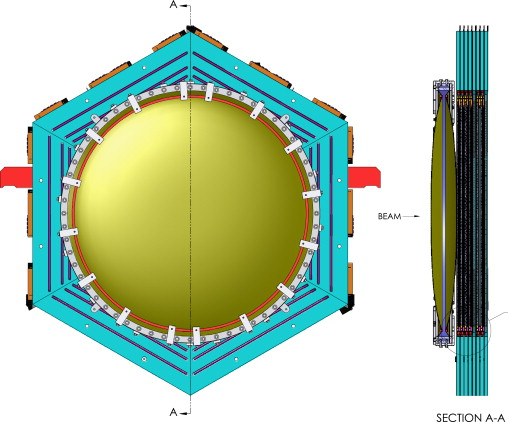
\includegraphics[scale=0.6]{Figures/Chapter2/WaterTarget.jpg}
        \caption{Scheme of the water target. Image from \cite{ALIAGA2014130}.}
        \label{fig:MnvExp:MnvDetector:WaterTarget}
    \end{figure}

    
    \item \textit{Active Tracker Region}
    
    The active tracker region consist of 61 tracker modules, giving a total of 122 tracking planes. This region the ID volume is filled completely of plastic scintillator, described in \ref{Cap:MnvExp:MnvDetector:ActiveTrackingPlanes}, and the OD volume consist of the ECAL and HCAL.
    
    \item \textit{Electromagnetic and Hadronic Calorimeter modules}
    
    The ID ECAL is located upstream the tracker region. The configuration of the planes in the ECAL region is similar to the tracker region, except that each plane has a 0.2 cm thick layer of lead embedded to the upstream side of the plane. This layer helps to stops the electrons and photons produced in the interaction vertex, obtaining a good energy resolution and directional information. This region contains 10 of this modules. 

    For the case of the ID HCAL, it has a similar configuration that the tracker region, but it has an steel plane of 2.54 cm thick each two planes, that is, each module has one steel plane. In the same way that the ECAL but with heavier particles, it allow a good energy resolution and directional information of particles such as protons and neutrons. 
    
\end{itemize}

\subsection{MINOS Near Detector}
\label{Cap:MnvExp:MnvDetector:MINOS}

The MINER$\nu$A detector is situated 2.1 m from the MINOS Detector and is used by MINER$\nu$A as muon spectrometer. The MINOS Near detector is designed to measure the muon neutrino flux close to the NuMI beam, performing a precise measurement in neutrino oscillation parameters for the muon neutrino disappearance. The MINOS Near detector is a magnetized tracking calorimeter composed of planes of plastic scintillator an iron giving a total mass of 1 kTon \cite{MINOSpaper}. The rectangular coil produce a toroidal magnetic field of a average strength of 1.3 T.

\begin{figure}
    \centering
    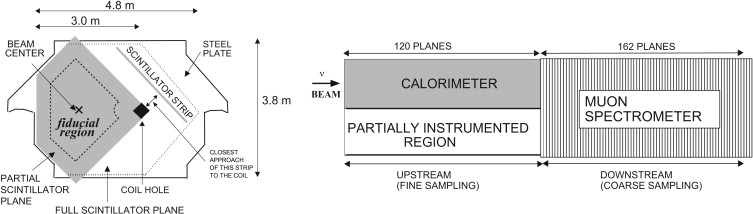
\includegraphics[scale=0.9]{Figures/Chapter2/MINOSNDScheme.jpg}
    \caption{Scheme of the lateral and frontal view of the MINOS Near detector. Some of the main components of the detector are shown. Figure from \cite{ALIAGA2014130}.}
    \label{fig:MnvExp:MnvDetector:SchemeMINOSND}
\end{figure}

The MINOS detector is able to measure the energy of the muon by the curvature or by range. The reconstruction by range is applied when the muon is contained in the detector measuring the ionization energy in the plastic scintillator and adding the correction for the passive steel. For the cases where the muon is not contained in the detector, the energy is reconstructed by the curvature of the track of the muon deflected by the magnetic field in MINOS. The energy measured by range is more precise that by curvature, for that it is preferred in the case that it is reconstructed by the two methods. For the reconstruction of the total muon energy, the energy measured by MINOS is added to the deposited energy of the muon in MINER$\nu$A. 


\begin{figure}[!htb]
    \centering
    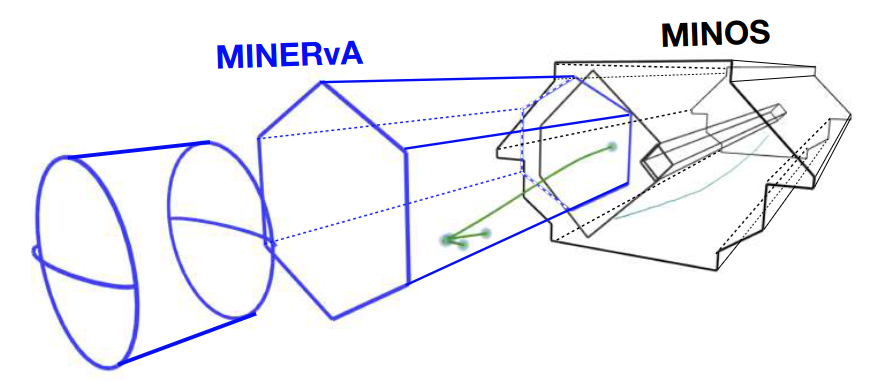
\includegraphics[scale=0.4]{Figures/Chapter2/MnvMINOS.png}
    \caption{Scheme that shows the volume of the He target, ID volume and the MINOS detector. In the scheme is shown how the MINER$\nu$A detector is aligned to the fiducial region of the MINOS detector. Image from \cite{MarvinThesis}.}
    \label{fig:MnvExp:MnvDetector:WholeMINERvADet}
\end{figure}

\subsection{Photodetection System}
\label{Cap:MnvExp:MnvDetector:PhotoDetectionSystem}

The light produced in the scintillator is downshifted by a wavelength shifting (WLS) fiber that is located in the center of the scintillator strip. The end of this fiber is polished to mirror level. The end of the cables are encrusted to optical connectors from Fujikura-DDK \cite{OpticalConnector}. Each connector holds 8 fibers in a linear shape. The connectors are referred to the other DDK connector, this connector holds 8 clear polished fibers. This cables transmit the light from the WLS to the photo-multipliers (PMT) boxes. All the WSL were tested checking the attenuation at different distances of the fiber and for the clear fibers were tested measuring the transmission of light. These procedures are described in \cite{ALIAGA2014130}.

\begin{figure}[!htb]
    \centering
    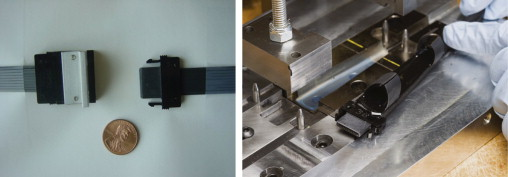
\includegraphics{Figures/Chapter2/OpticCablesConnectors.jpg}
    \caption{In the left, picture of the DDK connector. In the right the process of attach of the optical wires to the DDK connectors. Figure from \cite{ALIAGA2014130}.}
    \label{fig:MnvExp:MnvDetector:DDKConnector}
\end{figure}

The optical box consists in a frame that contains the Fiber-end Face plate, the cookie, the PMT, FEB connector board, two imputs for the Light Injection (LI) system, connecting cables and the Optical Decoder Unit (ODU). The ODU is an array that connects the Fiber-end face plate to the PMT. In the \textbf{Figure} \ref{fig:MnvExp:MnvDetector:OpticalBox} the components of the Optical box are shown. 

\begin{figure}[!htb]
    \centering
    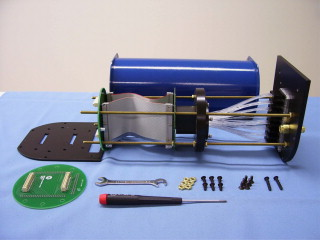
\includegraphics{Figures/Chapter2/OpticaBox.jpg}
    \caption{Picture where the internal components of the optical box. Figure from \cite{ALIAGA2014130}.}
    \label{fig:MnvExp:MnvDetector:OpticalBox}
\end{figure}

The photo-multipliers, more commonly known as PMTs, are sensitive light detectors that transform the light that is collected by the sensitive region in to an electric signal. The physics beyond the PMT is based on the photo-electric effect, when the photons pass through the input window and interacts with a  cathode it produce photo-electrons, these are accelerated by an electric field produced by a dynodes chain where the electrons collide producing a positve gain in the number of electrons. This technology allows to have information of the initial number of photons given the multiplicative factor of charge, the size of the signal is related with the deposited energy of the particles on the scintillator. 

\begin{figure}[!htb]
    \centering
    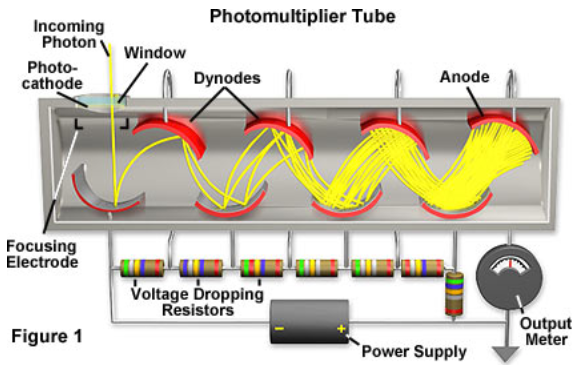
\includegraphics[scale=0.5]{Figures/Chapter2/PMT.png}
    \caption{Scheme where the functionality of a PMT is shown. In the image the mainly components of a PMT are shown. Figure from \cite{PMTHamamatsu}.}
    \label{fig:MnvExp:MnvDetector:PMTfunctionality}
\end{figure}



The PMT's model used is H8804MOD-2 manufactured by Hamamatsu Photonics \cite{hamamatsu2007photomultiplier}. The H8804MOD-2 PMT has an 8$\times$8 matrix of 2 mm $\times$ 2 mm pixels, giving a total of 64 pixels. The quantum efficiency required is 12\% at 520 nm and a maximum-to-minimum pixel gain  The spectral response of the PMT is 300-650 nm.    

The ODU has as main goal to separate physically the signal from adjacent scintillator strips, in the way that these are not adjacent pixels in the PMT. This distribution helps to reduce the cross-talk efects that can be presented in the plastic bars. In the \textbf{Figure} \ref{fig:MnvExp:MnvDetector:ODU} a diagram of the fibers pater is shown. 

\begin{figure}[!htb]
    \centering
    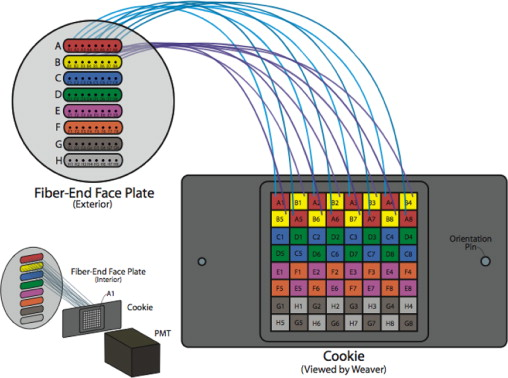
\includegraphics{Figures/Chapter2/ODU.jpg}
    \caption{Pattern of distribution of the fibers for each PMT. Figure from \cite{ALIAGA2014130}.}
    \label{fig:MnvExp:MnvDetector:ODU}
\end{figure}

Each optical box has two inputs for the light injection system (LI). This system consist in a light box that produce a blue pulsed light that is sent by two clear optical cables to each optical boxes, inside of the optical boxes the light is distributed uniformly over all the PMT pixels. The LI system turns on during ones after each beam spill. In this test the gain of the PMTs is measured and is used to monitoring the gain of the PMTs dearly. 

The output of the PMTs are connected to an electronic board know as front-end board (FEB). This electronic board digitize the analogical height and timing pulse that comes from the PMTs, provides a high voltage (HV) to the PMT and it send the digitized information to the Data Acquisition System (DAQ). 

\begin{figure}
    \centering
    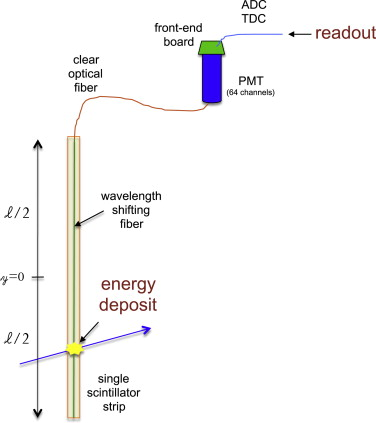
\includegraphics{Figures/Chapter2/OpticalSystem.jpg}
    \caption{Scheme that shows the meanly components of the optical system. It shows how the light travels from the plastic scintillator strips to the optical box. Figure from \cite{ALIAGA2014130}.}
    \label{fig:enter-label}
\end{figure}

\subsection{Calibration}
\label{Cap:MnvExp:MnvDetector:Calibration}

\subsection{Data Reconstruction}
\label{Cap:MnvExp:MnvDetector:DataReconstruction}

\subsubsection{Untracked pions reconsttruction}
\label{Cap:MnvExp:MnvDetector:DataReconstruction:Untrackedpions}
\textcolor{red}{Hablar sobre la reconstruccion para los untracked pions}

\subsection{Data Acquisition System }
\label{Cap:MnvExp:MnvDetector:DAQ}

The Data Acquisition System has a main roll collect all the information generated in the neutrino interaction and save it. 

After that the light is produced in the plastic scintillator strips, is explained in the \textbf{Subsection} \ref{Cap:MnvExp:MnvDetector:ActiveTrackingPlanes}, the light is carried by the 







